\documentclass[TFM.tex]{subfiles}

\begin{document}





\chapter{Proof of Deligne Conjecture}

 %PUEDE ESTAR BIEN INTRODUCIR LA HOMOTOPY G-ALGEBRA AUNQUE IGUAL ES UN POCO REDUNDANTE.  (COMPARAR LA DEFINICIÓN COMO BRACE ALGEBRA CON LA DE ALGEBRAIC OPERADS O LA QUE SEA QUE TENGO CITADA POR AHÍ)

Now that we know the equivalence $C_*(E_2)\simeq H_*(E_2)$, we can prove the Deligne conjecture if we find an action of an operad equivalent to $H_*(E_2)$ on the Hochschild complex $C^*(A;A)$ inducing the Gerstenhaber algebra structure on $H^*(A;A)$. In this chapter, we will denote $G=H_*(E_2)$. For any operad $\OO$ of a certain kind that we will call \emph{quadratic}, there is an operad $\OO_\infty$ and a map $\OO_\infty\to\OO$, which is a quasi-isomorphism under certain conditions that $G$ satisfies, so we have a quasi-isomorphism $G_\infty\to G$. From this point, the idea is to factor this map through
\[
G_\infty\to \BB,\BB\to G
\]
where $\BB$ is an operad which acts on $C^*(A;A)$ inducing the Gerstenhaber algebra structure on $H^*(A;A)$.  This factorization won't be constructed explicitly since it relies on an isomorphism of operads $\widetilde{\BB}\cong\BB$, which is obtained using tools of Etingof-Kazhdan quantization theory \cite{EK} (see also Section 7 of \cite{Hinich}). Finally, since $G_\infty\simeq G$ and $G_\infty\to\BB$ induces an action of $G_\infty$ on $C^*(A;A)$ via $\BB$, we have found an operad equivalent to the chain operad of little disks acting on the Hochschild complex and inducing the Gerstenhaber algebra on cohomology. 

Throughout this chapter $k$ is a field of characteristic 0. 


\section{Cooperads and coalgebras}

%EL LEMA 2.1 CREO QUE ES EL 5.1.3 DE COMPOSITION OPERADS, NO SÉ SI LO NECESITARÉ 

In order to define $G_\infty$ we need some general constructions. Most of the following definitions can be found in \cite{Hinich}. 

Let $\mathscr{M}$ be a monoidal category that admits indinite direct sums and the tensor product commutes with finite direct sums (usually $\mathscr{M}=\Vect, \Vectgr,\Ch$, where the vector spaces are considered to be finite dimensional). For a graded vector space $X=\bigoplus_{n\in\Z}X_n$, let us write $X[p]=\bigoplus_{n\in\Z}X_{n+p}$. We have for graded vector spaces $X$ and $Y$ that $X[p]\otimes Y[q]\cong (X\otimes Y)[p+q]$ and a map of degree $X\to Y$ of degree $n$ induces a map $X\to Y[n]$ of degree 0. 

\begin{defi}
 An \emph{$\mathbb{S}$-object} in $\mathscr{M}$ is a collection $X=\{X(n)\}_{n\geq 0}$ of objects of $\mathscr{M}$ endowed with a right action of the symmetric groups $\Sigma_n$.
\end{defi}

Note than an operad $\OO$ is just an $\mathbb{S}$-object endowed with
equivariant operations
\[\OO(k)\otimes\OO(j_1)\otimes\cdots\otimes\OO(j_k)\to \OO(j_1+\cdots+j_k)\]
and with a unit element $1 \in\OO$ satisfying natural associativity and unit conditions.




One has a forgetful functor from the category of operads to the category of $\mathbb{S}$-objects. This functor admits a \emph{free operad functor} as left adjoint \cite{GJ}. The free operad on an $\mathbb{S}$-object $X$ is denoted $\T(X)$ and can be thought as the operad generated by all formal operations corresponding to elements of each $X(n)$ and no relations between them (apart from the relations coming from the definition of operad). An explicit description is constructed in \cite{GJ} and alternatively in \cite{AlgebraicOperads}. Here we define $\T(X)$ by the usual universal property of free objects in a category. 

\begin{defi}
The \emph{free operad} over the $\mathbb{S}$-object $X$ is an operad $\T(X)$ equipped with an $\mathbb{S}$-object morphism $\eta(X):X\to\T(X)$ which satisfies the following universal condition: any $\mathbb{S}$-object morphism $f:X\to \OO$, where $\OO$ is an operad, extends uniquely into an operad morphism $\widetilde{f}:\T(X)\to\OO$ making the following diagram commute
\[
\begin{tikzcd}
X\arrow[r, "\eta(X)"]\arrow[dr,"f"] & \T(X)\arrow[d, "\widetilde{f}"]\\
& \OO
\end{tikzcd}
\] 
\end{defi}

Since the notions of operad and algebra over an operad can be defined in purely categorical terms, they can be dualized. Thus, a cooperad in $\mathscr{M}$ is the same as an operad in the opposite category $\mathscr{M}^{op}$. Similarly one defines a coalgebra over a cooperad. In particular, there is a categorical definition of $k$-algebra since $k$-algebras are algebras of vector spaces over the unital non-$\Sigma$ operad generated by one 0-ary operation (the unit) and one associative binary operation, but let us recall the definition of a coalgebra.

\begin{defi}\label{coalgebra}
A \emph{coalgebra} over a field $k$ is a vector space $V$ together with $k$-linear maps $\Delta:V\to V\otimes V$ and $\varepsilon:V\to k$ such that the following diagrams commute
\[
\begin{tikzcd}
V \arrow[r, "\Delta"] \arrow[d, "\Delta"'] & V\otimes V \arrow[d, "Id\otimes\Delta"] & V \arrow[r, "\Delta"] \arrow[d, "\Delta"'] \arrow[rd, "Id"] & V\otimes V \arrow[d, "Id\otimes\varepsilon"] \\
V\otimes V \arrow[r, "\Delta\otimes Id"]   & V\otimes V\otimes V                     & V\otimes V \arrow[r, "\varepsilon\otimes Id"]               & k\otimes V\cong V\cong V\otimes k           
\end{tikzcd}
\]
\end{defi}

\begin{ex}\label{cofree}
Maybe the most canonical example of coalgebra is the coalgebra structre on the tensor algebra $TW=\bigoplus_{n=0}^\infty W^{\otimes n}$ for a vector space $W$. The map $\varepsilon$ is just the projection onto the first coordinate. The comultiplication (or coproduct) $\Delta$ is defined on homogeneous elements as
\[
\Delta(w_1\otimes\cdots\otimes w_n)=\sum_{p=0}^n(w_0\otimes\cdots \otimes w_p)\otimes (w_{p+1}\otimes\cdots\otimes w_n).
\]
Note that $$\Delta(w_1\otimes\cdots\otimes w_n)\in\bigoplus_n\bigoplus_{p+q=n}W^{\otimes^n}=\bigoplus_{p,q}\left(W^{\otimes p}\otimes W^{\otimes q}\right)=\left(\bigoplus_p W^{\otimes p}\right)\otimes \left(\bigoplus_q W^{\otimes q}\right).$$ 

One easily checks that these maps make the diagrams in definition \ref{coalgebra} commute.
\end{ex}

In the previous example, it is clear that $\Delta^{n+1}(w_1\otimes\cdots\otimes w_n)=0$ (by abuse of notation the $n$-fold tensor product by the identity map is omitted). This condition means that $TW$ is a \emph{conilpotent} coalgebra. There is also a notion of conilpotency for coalgebras over cooperads expressed by the equation
\[
X=\bigcup_n\ker(X\to \DD(n)\otimes X^{\otimes n})
\]
for a cooperad $\DD$. In the same way that $TW$ is known to be the free associative algebra over $X$, with the coproduct given above it is the cofree (conilpotent) coalgebra cogenerated by $W$ \cite[Proposition 2.1 of \textsection 1.2.6]{AlgebraicOperads}.

Sometimes one has at the same time an algebra and a coalgebra structure on some graded vector space. Both structure might be compatible in the following sense.

\begin{defi}
A \emph{bialgebra} on vector space $V$ is a tuple $(V,\nabla,\eta, \Delta,\varepsilon)$, where $\nabla:V\otimes V\to V$ is the product and $\eta:k\to V$ is the unit that turn $X$ into a $k$-algebra, and where $\Delta$ and $\varepsilon$ are the coproduct and counit that turn $V$ into a $k$-coalgebra. This data must satisfy the following compatibility conditions:
\begin{enumerate}
\item $\cdot$ and $\Delta$ are compatible, i.e., the following diagrams commute
\[
\begin{tikzcd}
V\otimes V \arrow[r, "\nabla"] \arrow[d, "\Delta\otimes\Delta"'] & V \arrow[r, "\Delta"] & V\otimes V                                                    \\
V\otimes V\otimes V\otimes V \arrow[rr, "Id\otimes B\otimes Id"] &                       & V\otimes V\otimes V\otimes V \arrow[u, "\nabla\otimes\nabla"]
\end{tikzcd}
\]
where $B:V\otimes V\to V\otimes V$ is the braiding $B(x\otimes y)=y\otimes x$. 

\item $\nabla$ and $\varepsilon$ are compatible
\[
\begin{tikzcd}
V\otimes V \arrow[r, "\nabla"] \arrow[d, "\varepsilon\otimes\varepsilon"'] & V \arrow[ld, "\varepsilon"] \\
k\otimes k\cong k                                                          &                            
\end{tikzcd}
\]
\item $\Delta$ and $\eta$ are compatible
\[
\begin{tikzcd}
k\otimes k\cong k \arrow[d, "\eta\otimes\eta"'] \arrow[rd, "\eta"] &                       \\
V\otimes V                                                         & V \arrow[l, "\Delta"]
\end{tikzcd}
\]
\item $\eta$ and $\varepsilon$ are compatible
\[
\begin{tikzcd}
k \arrow[rd, "\eta"] \arrow[d, "Id"'] &                            \\
k                                     & V \arrow[l, "\varepsilon"]
\end{tikzcd}
\]
\end{enumerate}

\end{defi}

\begin{ex}
There is another coalgebra structure on $TW$ that behaves better with the algebra structure in the sense defined above. One defines $\Delta:TW\to TW\otimes TW$ by linear extension of $\Delta(w)=w\otimes 1+1\otimes w$ for $w\in W$ and $\Delta(1)=1\otimes 1$. The same $\varepsilon$ as in example \ref{cofree} is valid. The multiplication is simply $\nabla(x\otimes y)=x\otimes y$ and the unit is the inclusion $\eta:k\to TW$. It is tedious but straightforward to check all the compatibilities, since it is enough to do it for elements of $W$. 
\end{ex}

%creo que el dual de epsilon en el caso de las álgebras sería k-> X=X\otimes k, o sea, la multiplicación por escalar en el producto tensorial
%LO DE NILPOTENTES CREO QUE NO LO NECESITO




%EL SIGMA AHÍ QUÉ ES, APLICACIONES DESDE $\Sigma_n$ SERÍA COMPATIBLE CON EL CASO $N=1$ MÁS ADELANTE, PERO NO SÉ SI ES ESO
%
%EN LAS RELACIONADAS HAY COSAS QUE PUEDEN SER INTERESANTES (Y ALOMEJOR NECESITO AÑADIR LO DE NILPOTENT \url{https://math.stackexchange.com/questions/157071/understanding-cofree-coalgebras?rq=1}) \url{https://math.stackexchange.com/questions/3204571/notation-involving-the-symmetric-group-s-n?noredirect=1#comment6593463_3204571}
%
%PÁGINA 130 DE ALGEBRAIC OPERADS SON LOS INVARIANTES BAJO LA ACCIÓN


\begin{defi}
Let $\OO$ be an operad in $\mathscr{M}$. Let $X$ be an $\mathbb{S}$-object in $\mathscr{M}$. The free $\OO$-algebra generated by $X$ is defined to be
\[
\F_\OO(X)=\bigoplus_{n\geq 0}\OO(n)\otimes_{\Sigma_n}X^{\otimes n}
\]
with a canonical $\OO$-algebra structure that we explain next. Here, $X^{\otimes n}$ is viewed as a left $\Sigma_n$-module under the left action 
\[
\sigma\cdot(v_1,\dots, v_n)=(v_{\sigma^{-1}(1)},\dots,v_{\sigma^{-1}(n)}).
\]
The structure maps $\OO(n)\otimes\F_\OO(X)^{\otimes n}\to \F_\OO(X)$ are given on each direct summand  by maps
\[
\OO(n)\otimes\OO(p_1)\otimes_{\Sigma_{p_1}} X^{\otimes p_1}\otimes\cdots\otimes \OO(p_n)\otimes_{\Sigma_{p_n}} X^{\otimes p_n}\to \OO(p_1+\cdots+p_n)\otimes_{\Sigma_{p_1+\cdots+p_n}}V^{\otimes p_1+\cdots+p_n}
\]
where an element $x_0\otimes x_1\otimes v_1\cdots v_{p_1}\otimes x_2\otimes v_{p_1+1}\cdots v_{p_1+p_2}\otimes \cdots\otimes x_n\otimes v_{p_1+\cdots+p_{n-1}+1}\cdots v_{p_n}$ is sent to $(-1)^{\varepsilon} x_0(x_1,\dots, x_n)\otimes v_1\otimes\cdots\otimes v_{p_1+\cdots+p_n}$. Here, $\varepsilon$ represents an exponent in which $|v_j|$ is added for each $x_i$ that was initially written at the right of $v_j$. 

\end{defi} 

For coalgebras over cooperads there is also a notion of cofree coalgebra. 

\begin{defi}
If $X$ is an $\mathbb{S}$-object in $\mathscr{M}$ and $\DD$ a cooperad in $M$. The \emph{cofree coalgebra cogenerated by }$X$ is defined to be
\[
\F^*_\DD(X)=\oplus_{n\geq 0}\left(\DD(n)\otimes X^{\otimes n}\right)^{\Sigma_n}
\]
where the subperscript $\Sigma_n$ stands for the invariant elements under the action of $\Sigma_n$ and the structure maps are dual to those in the free algebra. %como son invariantes, los elementos de V^n tienen que ser los de la diagonal, así que de una ristra de v se divide en los trozos que hacen falta y en la parte de D(n) simplemente se opera con la estructura de cooperad, posiblemente con algún signo también de saltar cosas. Para que no haya infinitos que sean 0 quizá vale con dejar de hacer copias en n=grado del elemento que estás copiando o algo así. A veces se considera el producto directo para no tener que preocuparse.
\end{defi}



Let $X$ be a $\DD$-coalgebra and $X$ be an $\mathbb{S}$-object. Any map $X\to V$ of $\mathbb{S}$-objects defines canonically a map of $\DD$-coalgebras $X\to \F_\DD^*(V)$.  

The cofree cooperad cogenerated by $X$ is denoted $\T^*(X)$, and it is isomorphic to $\T(X)$ as an $\mathbb{S}$-object. 

\begin{remark}\label{dual}
Let $\OO$ be an operad of graded vector spaces such that the $\OO(n)$ are all finite dimensional. The, the collection of dual spaces $\{\OO(n)^*\}$ has an obvious cooperad structure. This cooperad is denoted $\OO^*$. Coalgebras over $\OO^*$ are sometimes called $\OO$-coalgebras. In the same style, we will sometimes write $\F^*_\OO(X)$ instead of $\F^*_{\OO^*}(X)$ since this object is a coalgebra over a cooperad, and therefore there is no confusion.
\end{remark}

\begin{defi}
An operad $\OO$ of graded vector spaces is called \emph{quadratic} if it is generated as an operad by $\OO(2)$ and relations spanned by composition of two binary operations (equivalently, the set of relations lies in $\OO(3)$). 
\end{defi}

In chapter \ref{3} we explained that $G=H_*(E_2)$ was generated by $G(2)=H_*(E_2(2))$ and their relations involved compositions of $\mu$ and $l$ as we saw in the previous chapter. This shows that $G$ is quadratic. %en cada composición intervienen 2, no hay una tirple composición

\begin{defi}
Let $\OO$ be a quadratic operad with $V=\OO(2)$ and space of relations $R$. The \emph{dual cooperad} $\OO^{\perp}$ is cogenerated by the space $V[1]$ with corelations $R[2]$.
\end{defi}

%Let us explain this definition. Consider the quadratic operad of finite dimensional vector spaces generated by $V$ and relations $R$. Define $\widetilde{\OO}$ to be the operad generated by $V[1]^*\cong V[1]$ and relations $R^\perp=\{\varphi\in (V[1]\otimes V[1])^*=V[2]^*\mid R\subseteq\ker\varphi\}$. Then one defines $\OO^\perp=\widetilde{\OO}^*$ 

\begin{defi}
Let $\OO$ be a (graded) quadratic operad. A structure of $\OO_\infty$-operad on $X\in\Vectgr$ is given by a differential on the cofree $\OO^\perp$-coalgebra cogenerated by $X$.
\end{defi}

The above definition gives rise to an operad $\OO_\infty$ in the category of complexes of graded vector spaces over $k$ that can be realized as $\T(\OO^\perp)$ \cite{Hinich}. 
%In the case of $G_\infty$-algebras, there is an explicit definition than can be found in \cite[Proposition 16]{Galvez}. SI ME DA TIEMPO PONERLA EN ALGÚN LAO, AUNQUE REQUIERE VARIAS COSAS PREVIAS COMO TENGO POR AHÍ ABAJO EN MAYÚSCULAS COMENTADO


%Let $X$ have a structre of $\OO_\infty$-algebra. The differential
%\begin{equation}\label{9}
%Q:\F^*_{\OO^\perp}(X)\to \F^*_{\OO^\perp}(X)[1]
%\end{equation}
%is defined uniquely by its composition with the projection onto the degree one component $\F^{*1}_{\OO^\perp}(X)=X$. ¿POR QUÉ? Thus, the differential is given by the collection of maps
%\[
%Q_i:\F^{*i}_{\OO^\perp}(X)=(\OO^\perp(i)\otimes X^{\otimes i})^{\Sigma_i}\to X[1].
%\]
%In particular, $d=Q_1$ defines a differential on $X\in\Vectgr$. COMO EL DUAL ESTÁ SHIFTEADO EL DE 1 ES COMO SI FUERA EL DE 0 QUE ES K Y POR ESO SALE.
%
%Define $\OO_\infty=\T(\OO^\perp)$ to be the free graded operad generated by $\OO^\perp$ (as $\mathbb{S}$-object). The collection of
%maps $Q_i$ defines an action of $\OO_\infty$ on $X$. We have the following lemma ME GUSTARÍA UNA REFERENCIA PORQUE HINICH NI LO PRUEBA NI LO REFERENCIA, ADEMÁS LUEGO EN EL EJEMPLO DEFINE UNA DIFERENCIAL, PERO NO SABEMOS SI PARA ESA VALE QUE $Q^2=0$ IMPLIQUE QUE $Q$ RESPETA LAS DIFERENCIALES
%
%%LO DE LA DIFERENCIAL ME HACE FALTA PARA QUE LA APLICACIÓN RESPETE LAS DIFERENCIALES Y SEA DE VERDAD UN MORFISMO DE ALGEBRAS EN COMPLEJOS DE CADENAS
%Nextt, we have the following lemma.
%\begin{lemma}
%There exists a unique differential on the graded operad $\OO_\infty$ such that the condition $Q^2=0$ for a degree one differential $Q$ as in \ref{9} is equivalent to the statement that the action of $\OO_\infty$ on $(X,d=Q_1)$ respects the differentials. 
%\end{lemma}
%
%
%\begin{ex}
%Let $X$ be a complex endowed with a $\OO$-algebra structure (dg $\OO$-algebra). Define the differential $Q$ on $\F^*_{\OO^\perp}(X)$ as follows.
%
%$Q_1:X\to X[1]$ is the differential of $X$. $Q_2:\OO^{\perp}(2)\otimes X^{\otimes 2}\to X[1]$ is defined by the $\OO$-algebra structure on $X$ since $\OO^\perp(2)=\OO(2)[1]$. For $i>2$, $Q_i$ are defined to be 0. 
%
%The condition $Q^2=0$ can be easily verified since we're assuming that $\OO$ is quadratic. This means that any $\OO$-algebra admits a canonical $\OO_\infty$-algebra structure. 
%\end{ex}
%
%The last example shows that there is a canonical map of operads in $\Ch$
%\begin{equation}\label{map}
%\OO_\infty\to \OO.
%\end{equation}
%DICE HINICH QUE SUPONE QUE O TIENE DIFERENCIAL 0 PERO NO VEO LA NECESIDAD.
Using some technical results about dg-operads, Hinich shows that there is a map $\OO_\infty\to \OO$ for any quadratic operad. 

\begin{defi}
A quadratic operad $\OO$ is called \emph{Koszul} if the map $\OO_\infty\to \OO$ is a quasi-isomorphism.
\end{defi}

Hinich \cite{Hinich} shows that $G$ is Koszul using Kähler differentials and other techniques that we won't describe here. Another approach using that $G_\infty$ is the \emph{Koszul resolution} of $G$ is presented in \cite{AlgebraicOperads}. That fact is also proved in \cite{GJ}. In any case, we have a  quasi-isomorphism %(indeed, an homotopy equivalence \cite{strong})
\begin{equation}\label{equivalence}
G_\infty\xrightarrow{\simeq} G.
\end{equation}
The operad $G_\infty$ is called the operad of \emph{homotopy Gerstenhaber algebras}. This should not be confused with another \emph{homotopy G-algebra} found in the literature (\cite{VO} and \cite{VGH} for example) that will be briefly explained later. 

%AQUÍ LO QUE PUEDA SACAR DE HINICH

%\url{https://en.wikipedia.org/wiki/Bialgebra}
%
%\url{https://en.wikipedia.org/wiki/Coalgebra}

%SECCIÓN 5.5 (CREO QUE PUEDO ESQUIVAR LO DE DG BIALGEBRA DANDO DIRECTAMENTE LA ESTRUCTURA EN EL GRADED VECTOR SPACE)

%CREO QUE DE 6 ME LO PUEDO SALTAR, PORQUE AUNQUE CONSTRUYE LA APLICACIÓN, REQUIERE LAS CONSTRUCCIONES RARAS DEL PRINCIPIO (SALVO QUE EN ALGÚN MOMENTO LAS ENTIENDA, TIENEN UNA DESCRIPCIÓN EXPLÍCITA EN LAS PÁGINAS 5-6 PERO NO SÉ QUÉ REPRESENTA $S_n$ EN CADA CASO) ASÍ QUE SOLO COMENTAR QUE HACE FALTA LO DE ETINGOF-KAZHDAN


%EN ALGUNO DE LOS PAPERS PONE QUE KOSZUL ES CUANDO ES CUADRÁTICA (GENERADA POR LA OPERACIÓN DE GRADO 2) Y LAS RELACIONES ESTÁN EN $V\oplus (V\otimes V)$ ASÍ QUE ENTIENDO QUE VALENCIA 0 ES EN EL CUERPO Y POR ESO VALENCIA 3 ES AHÍ

%QUIÉN COÑO ES $G_\infty$? ¿ES SIMPLEMENTE PONERLE EL INFINITO COMO EN 3.1.4 (PARA LO CUAL TENGO QUE ENTENDER MEJOR LAS CONSTRUCCIONES ESAS DE MIERDA)? (Y DE ALGÚN MODO SALE EL OPERAD, QUIZÁ POR LO QUE SE CUENTA ANTES COMO LAS CONMUTATIVAS Y LAS ASOCIATIVAS Y LAS LIE) EN ESE CASO EL EJEMPLO 3.1.7 DARÍA YA UNA APLICACIÓN $G_\infty\to G$ PERO SUPONGO QUE HAY QUE DE TODOS MODOS HAY QUE PROBAR QUE SE TIENE UNA APLICACIÓN QUE ES EQUIVALENCIA

%---------------------------------------------------------------------------------------------------------------------

%PARA DESCRIBIR $G_\infty$ (AUNQUE COMENTARÉ QUE SE PUEDE DESCRIBIR COMO LA RESOLUCIÓN DE KOSZUL DE $G$): GALVEZ-CARRILLO PROPOSITION 16 PAGINA 559 (21 DEL PDF). PRIMERO NECESITO LA DEFINICIÓN DE S DE LA CONVENCIÓN 0.1 EN LA PÁGINA 542 (4 DEL PDF), PARA LA BARRA PÁGINA 554 (16 DEL PDF). AUNQUE TENIENDO EN CUENTA QUE NO ME DA LA APLICACIÓN A $G$, CREO QUE ME TRAE MÁS CUENTA TRATAR DE HACERLO COMO HINICH, QUE NO ES TAN COMPLICADO DE DEFINIR, SOLO DE ENTENDER, PERO CREO QUE PUEDO (Y COMENTAR QUE EN GALVEZ-CARRILLO ESTÁ MÁS EXPLÍCITO)

%LA PROPIEDAD DE QUE SEA UN QUASISOMORFISMO ES PARA QUADRATIC OPERAD (ALGEBRAIC OPERADS 7.1.1)

\section{Operad $\BB$ and its action on the Hochschild complex}
We shall now describe an operad which acts naturally on the Hochschild complex of any associative algebra inducing the Gerstenhaber algebra structure on cohomology. This operad is
usually denoted $\BB_\infty$ (see \cite{Hinich} and \cite{VO}), but since it is not obtained by Koszul resolution of any operad $\BB$ and to avoid confusion with the $B_\infty$-operad defined in chapter \ref{4}, we will denote it $\BB$. 

\begin{defi}
A $\BB$-algebra structure on a graded vector space $X$ is given by a structure of dg bialgebra on the tensor coalgebra $TX[1]=\bigoplus_{n=0}^\infty X[1]^{\otimes n}$ so that the coalgebra structure is the standard cofree one.
\end{defi}

Let us check that a $\BB$-algebra structure is given by an operad that will be denoted $\BB$. 
%PREGUNTAR POR LAS TRANSFORMACIONES QUE HACE PARA LLEGAR A LA DEFINICIÓN QUE ESTOY PONIENDO PORQUE IGUAL NO TIENE SENTIDO DECIR QUE LAS QUE SALEN SON DIFERENTIAL DE GRADO 1
The dg bialgebra structure on $TX[1]$ by the following data:
\begin{itemize}
\item a differential $D:TX[1]\to TX[1]$ which decomposes on maps $X[1]^{\otimes n}\to X[1]^{\otimes r}$ of degree 1. The differential is uniquely defined by its $r=1$ part since it must be compatible with the coproduct. We denote its $(n,1)$-componets by $m_n:X[1]^{\otimes n}\to X[2]$ or, what is the same, 
\begin{equation}\label{mn}
m_n:X^{\otimes n}\to X[2-n].
\end{equation}
%Sería D:TX[1]->TX[1] pero se puede restringir a cada componente

\item a multiplication $M:TX[1]\otimes TX[1]\to TX[1]$ which decomposes on maps $X[1]^{\otimes p}\otimes X[1]^{\otimes q}\to X[1]^{\otimes r}$ of degree 0 since the tensor product commute with infinite sums. It is also defined by its $r=1$ part. We denote the collection of $r=1$ multiplications by $m_{pq}:X^{\otimes p}[1]\otimes X^{\otimes q}[1]\to X[1]$ or, what is the same, 

\begin{equation}\label{mpq}
m_{pq}:X^{\otimes p}\otimes X^{\otimes q}\to X[1-p-q].
\end{equation}
%Aquí lo mismo, teniendo en cuenta que en R-Mod las sumas directas infinitas conmutan con el producto tensorial, luego TX[1]xTX[1] se puede definir en cada componente
\end{itemize}
Therefore, the $\BB$-structure is given by a collection of operations $m_n$ and $m_{pq}$
subject to some relations. This defines an operad $\BB$ as the one generated by $m_n\in\BB(n)_{2-n}$ and $m_{pq}\in\BB(p+q)_{1-p-q}$ subject to some relations. More precisely, the relations are given by $D^2=0$, associativity of $M$, the Leibniz rule and the usual compatibility relations between this algebra structure with the cofree coalgebra structure on $TX[1]$. We're going to explicitly write down some of these conditions since they are needed to to show that $\BB$ acts on $C^*(A;A)$.  %ESCRIBIR LAS RELACIONES CON 2.2 DE VORONOV

For that purpose, let us introduce the following notation from \cite{VO}. For an element $a_1\otimes\cdots\otimes a_n\in V[1]^{\otimes n}$, write
\[
m_n(a_1,\dots,a_n)=(-1)^{(k-1)|a_1|+(k-2)|a_2|+\cdots+|a_{n-1}|}m_n(a_1\otimes\cdots\otimes a_n),
\]
which morally means that the vertical bar $|$ has degree one and on the left-hand
side all the bars are moved between $m_n$ and $a_1$. However, we set
\[
m_{pq}(a_1,\dots, a_p;b_1,\dots, b_q)=m_{pq}((a_1\otimes\cdots\otimes a_p)\otimes(b_1\otimes\cdots\otimes b_q)).
\]

The condition $D^2=0$ is equivalent to the following identity for every $r\geq 1$
\begin{equation}\label{6}
\sum_{i+j-1=r}\sum_{k=0}^{r-j}(-1)^\varepsilon m_i(a_1,\dots, a_k,m_j(a_{k+1},\dots, a_{k+j}),a_{k+j+1},\dots, a_r)=0
\end{equation}
where $\varepsilon=(i+1)j+(j+1)k+i|a_1|+(i-1)|a_2|+\cdots+(i-k+1)|a_k|+(n-k-1)|a_{k+1}|+(n-k-2)|a_{k+2}|+\cdots+|a_{n-1}|$ and $a_1,\dots, a_n\in X$. In fact, the sign $\varepsilon$ is obtained as $|a_1|+\cdots+|a_k|−k$ plus the sign coming from moving the vertical bars
in any occurrence of $M_p[a_1| \dots |a_p]$ to the place between $M_p$ and $a_1$, thinking of a
bar as having degree 1.

The associativity of $M$ is equivalent to the followint identities
\begin{equation}\label{7}
\begin{aligned}
\sum_{r=1}^{l+t}\underset{t_1+\cdots+t_r=t}{\sum_{l_1+\cdots+l_r=l}}&(-1)^{\varepsilon}m_{k,r}(a_1,\dots, a_k;m_{l_1,t_1}(b_1,\dots, b_{l_1};c_1,\dots, c_{t_1}),\\
&\dots, m_{l_r,t_r}(b_{l_1+\cdots+l_{r-1}+1},\dots,b_l;c_{t_1+\cdots+t_{r-1}+1},\dots,c_t))\\
=&\sum_{s=1}^{k+l}\underset{l_1+\cdots+l_s=l}{\sum_{k_1+\cdots+k_s=k}}(-1)^\delta m_{s,t}(m_{k_1,l_1}(a_1,\dots, a_{k_1};b_1,\dots, b_{l_1}),\dots,\\
&m_{k_s,l_s}(a_{k_1+\cdots+k_{s-1}+1},\dots, a_k;b_{l_1+\cdots+l_{s-1}+1},\dots,b_l);c_1,\dots, c_t)
\end{aligned}
\end{equation}
for $a_1,\dots, a_k,b_1,\dots, b_l,c_1,\dots, c_t\in X$. The sign $(-1)^\varepsilon$ is the sign picked up by reordering $[a_1|\cdots|a_k|b_1|\cdots|b_l|c_1|\cdots|c_t]$ into $$[a_1|\cdots|a_k|b_1|\cdots|b_{l_1}|c_1|\cdots|c_{t_1}|\cdots|b_{l_1+\cdots+l_{r-1}+1}|\cdots|b_l|c_{t_1+\cdots+t_{r-1}+1}|\cdots|c_t]$$ in the graded vector space $TX[1]$. 

Similarly, $(-1)^\delta$ is the sign of reordering $[a_1|\cdots|a_k|b_1|\cdots|b_l|c_1|\cdots|c_t]$ into $$[a_1|\cdots|a_{k_1}|b_1|\cdots|b_{l_1}|\cdots|a_{k_1+\cdots+k_{s_1}+1}|\cdots|a_k|b_{l_1+\cdots+l_{s-1}+1}|\cdots|b_1|c_1|\cdots|c_t].$$

Finally, the Lebniz rule of $D$ with respect to $M$ is equivalent to the following identities
\begin{equation}\label{8}
\begin{aligned}
\sum_{n=1}^{k+l}\underset{l_1+\cdots+l_n=l}{\sum_{k_1+\cdots+k_n=k}}&(-1)^\varepsilon m_n(m_{k_1,l_1}(a_1,\dots, a_k;b_1,\dots, b_l),\dots,\\
&m_{k_n,l_n}(a_{k_1+\cdots+k_{n-1}+1},\dots, a_k;b_{l_1+\cdots+l_{n-1}+1},\dots, b_l))\\
=&\sum_{r=1}^k\sum_{i=0}^{k-r}(-1)^\delta m_{k-r+1,l}(a_1,\dots, a_i,m_r(a_{i+1},\dots, a_{i+r}),\dots, a_k;b_1,\dots, b_l)\\
&+(-1)^{|a_1|+\cdots+|a_k|-k}\sum_{s=1}^l\sum_{i=0}^{l-s}(-1)^\eta m_{k,l-s+1}(a_1,\dots, a_k;b_1,\dots, b_i,\\
&m_s(b_{i+1},\dots, b_{i+s}),\dots, b_l)
\end{aligned}
\end{equation}

for $a_1,\dots , a_k,b_1, \dots , b_l \in X$. The sign $(−1)^\varepsilon$ is the sign of reordering $[a_1| \cdots |a_k|
b_1| \cdots |b_l]$ into $[a_1| \cdots |a_{k_1} |b_1| \dots |b_{l_1} | \cdots |a_{k_1+\cdots+k_{n−1}+1}|  \cdots |a_k|b_{l_1+\cdots+l_{n−1}+1}| \cdots |b_l]$
in $T X [1]$ multiplied by the sign of moving $n − 1$ bars between $m_{k_1,l_1}(\dots ),\dots ,m_{k_n,l_n}(\dots )$ to the place between $m_n$ and $m_{k_1,l_1}$. The sign $(−1)^\delta$ is equal to $|a_1|+\cdots+|a_i|−i$ plus the sign coming from moving the vertical bars in $m_r[a_{i+1}|\cdots|a_{i+r}]$
to the place between $m_r$ and $a_{i+1}$. Similarly, the sign $(−1)^\eta$ is equal to $|b_1|+\cdots+|b_i|−
i$ plus the sign coming from moving the vertical bars in $m_s[b_{i+1}|\cdots |b_{i+s}]$ to the
place between $m_s$ and $b_{i+1}$.
\subsection{Brace algebra}



Before specifying the action of $\BB$ on the Hochschild complex we need to introduce the following algebraic structure. References to this are \cite{VGH} and \cite{VO}.


\begin{defi}\label{braces}
On the graded vector space given by an operad $\OO=\bigoplus_n\OO(n)$ define the multilinear operators called \emph{braces}:
\[
x\{x_1,\dots, x_n\}=\sum(-1)^\varepsilon\gamma (x;1,\dots, 1,x_1,1,\dots, 1,x_n,1,\dots,1)
\]
for $x,x_1,\dots, x_n\in\OO$, where the summation runs over all possible substitutions of $x_1,\dots, x_n$ into $x$ in the prescribed order and $\varepsilon=\sum^n_{p=1}|x_p|i_p$, $ip$ being the total number of inputs in front of $x_p$. %ESTO PUEDO USARLO PARA EL OTRO SIGNO QUE TENÍA EN ALGUNA PARTE. 
\end{defi}

The braces $x\{x_1, \dots , x_n\}$ are homogeneous of degree $−n$, i.e., $|x\{x_1, \dots , x_n\}|=|x|+|x_1|+\cdots+|x_n|-n$. We will also assume the following conventions:
\[
x\{\}=x,\ x\circ y=x\{y\}.
\]

\begin{remark}
The sign is motivated by the example where $\OO = \End (V)$, the endomorphism
operad of a vector space $V$: $\End (V)(n) = \Hom(V^{\otimes n}, V)$. Then the sign $(−1)^\varepsilon$ is picked
up by rearranging the sequence of letters $x\{x_1, \dots , x_n\}(v_1, \dots , v_m)$, where $v_1, \dots , v_m ∈ V$,
and $m$ is such that $x\{x_1, \dots , x_n\} ∈ \Hom(V^{\otimes m}, V)$, into the sequence $γ(x; v_1, \dots , v_{i_1} ,x_1(v_{i_1+1}, \dots), \dots, v_{i_n}, x_n(v_{i_n+1}, \dots), \dots , v_m)$ in accordance with the usual sign convention.
\end{remark}

One can immediately check the following identities:

\begin{equation}\label{identity}
\begin{aligned}
&x\{x_1, \dots , x_m\}\{y_1, \dots , y_n\}=\\
&\sum_{0\leq i_1\leq\cdots\leq i_m\leq n}(-1)^\varepsilon x\{y_1,\dots, y_{i_1}, x_1\{y_{i_1+1},\dots\},\dots y_{i_m}, x_m\{y_{i_m+1},\cdots\},\dots, y_n\}
\end{aligned}
\end{equation}
where $\varepsilon =\sum^m_{p=1}(|x_p|-1)\sum^{i_p}_{q=1}(|y_q|-1)$, i.e., the sign is picked up by the $x_i$’s passing through the
$y_j$’s in the shuffle.


\begin{remark}
The identity (\ref{identity}) for $m=n=1$ implies that the degree 1 bracket
\[
[x,y]=x\circ y-(-1)^{(|x|-1)(|y|-1)}y\circ x
\]
defines the structure of a graded Lie algebra on $\OO$. Indeed, puting $m = n = 1$ in (\ref{identity}), one obtains 
$$x\{y\}\{z\} − x\{y\{z\}\} = x\{y, z\} + (−1)^{(|y|-1)(|z|-1)}x\{z, y\},$$ %salen dos términos a la derecha porque hay que pensar más bien en el espíritu de la fórmula, que es el de meter de todas las formas posibles
which measures the failure of the operation $(x, y) → x\{y\}$ to be associative.  Note that

$$x\{z\}\{y\} − x\{z\{z\}\}=x\{z, y\} + (−1)^{(|y|-1)(|z|-1)}x\{y,z\}=(-1)^{(|y|-1)(|z|-1)}(x\{y\}\{z\} − x\{y\{z\}\}).$$

Using the $\circ$ notation, this rewrites as
\begin{equation}\label{circ}
(x\circ y)\circ z-x\circ(y\circ z)=(−1)^{(|y|-1)(|z|-1)}((x\circ z)\circ y- x\circ (z\circ y)).
\end{equation}
Now, recall the graded Jacobi identity 

$$(-1)^{(|x|-1)(|z|-1)}[[x,y],z]+(-1)^{(|y|-1)(|x|-1)}[[y,z],x]+(-1)^{(|z|-1)(|y|-1)}[[z,x],y]=0$$

Using the notation of \cite[Theorem 1]{Gerstenhaber}, the first term is 
\[
(-1)^{\lambda\nu}[(x\circ y -(-1)^{\lambda\nu}y\circ x)\circ z-(-1)^{|\lambda+\mu|\nu}z\circ(x\circ y-(-1)^{\lambda\mu}y\circ x)],
\]

where $\lambda=|x|-1$, $\mu=|y|-1$ and $\nu=|z|-1$. Using (\ref{circ}), this is equal to
\[
(-1)^{\lambda\nu}[(x\circ y -(-1)^{\lambda\nu}y\circ x)\circ z-(-1)^{|\lambda+\mu|\nu}((z\circ x)\circ y-(-1)^{\lambda\mu}(z\circ y)\circ z)].
\]
Applying similar transformations to the other terms we get
\begin{gather*}
(-1)^{\lambda\nu}[(x\circ y -(-1)^{\lambda\mu}y\circ x)\circ z-(-1)^{(\lambda+\mu)\nu}((z\circ x)\circ y-(-1)^{\lambda\mu}(z\circ y)\circ z)]\\
+(-1)^{\mu\lambda}[(y\circ z -(-1)^{\mu\nu}z\circ y)\circ x-(-1)^{(\mu+\nu)\lambda}((x\circ y)\circ z-(-1)^{\mu\nu}(x\circ z)\circ y)]\\
+(-1)^{\nu\mu}[(z\circ x -(-1)^{\nu\lambda}x\circ z)\circ z-(-1)^{(\nu+\lambda)\mu}((y\circ z)\circ x-(-1)^{\nu\lambda}(y\circ x)\circ z)]
\end{gather*}
which vanished identically.
\end{remark}

\begin{defi}
A brace algebra is a graded vector space with a collection of braces
$x\{x_1,\dots , x_n\}$ of degree $−n$ satisfying the identities (\ref{identity}).
\end{defi}

Thus we have made the following observation.

\begin{prop}
For every operad $\OO$ of vector spaces, the braces define the natural
structure of a brace algebra on the underlying graded vector space $\OO$. \qed
\end{prop}

Now let $A$ be any associative $k$-algebra and $\CC=C^*(A;A)$. $\CC$ naturally becomes a brace algebra using its operadic structure. To avoid the unpleasant signs it is convenient to denote elements $f \in \CC^n$ as boxes having $n$ inputs and one output like this:

\begin{figure}[h!]
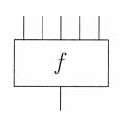
\includegraphics[scale=0.8]{Imagenes//box}
\end{figure}



Let $f,g_1,\dots, g_n\in \CC$. The the brace $f\{g_1,\dots, g_n\}$ is given by the following formula.\\

\begin{figure}[h!]
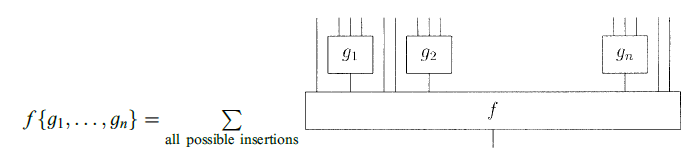
\includegraphics[scale=0.7]{Imagenes//brace}
\end{figure}

Here the sum is taken over all possible order preserving insertions of outpus of $g_i$ into
inputs of $f$.




The Lie bracket on $\CC$ is given explicitly, in terms of braces, by the formula %pone \CC[1] porque es de grado 1
\[
[f,g]=f\{g\}-(-1)^{(|f|-1))(|g|-1)}g\{f\}.
\]
and coincides with the one defined by Gerstenhaber in \cite{Gerstenhaber} (beware of the distinction between dimension and degree).
%en la sección 6 de Gerstenhaber sale la composición con la cual [f,g] es el conmutador, que consiste precisamente hacer las inserciones




\subsection{Action of $\BB$ on $C^*(A;A)$}
We have to define the action of the operations
$m_n$ (\ref{mn}) and $m_{pq}$ (\ref{mpq}) on $C^*(A;A)$ and to check the compatibilities. The action is given below.
\begin{itemize}
\item $m_0=0$.
\item $m_1$ is the differential $d$ in $\CC$. 
\item $m_2$ is the multiplication $m:\CC\otimes\CC\to\CC$ defined by the formula $m(x\otimes y)=x\smile y$, where $\smile$ is the usual cup product $(x\smile y)(a_1,\dots, a_{k+l})=x(a_1,\dots, k)y(a_{k+1},\dots, a_{k+l})$ for $x\in C^k(A;A)$, $y\in C^l(A;A)$ and $a_i\in A$. It will also be written just as $x\cdot y$ or $xy$ when there is no confusion.
\item $m_n=0$ for all $n>2$. 
\item $m_{0,1}=m_{1,0}=Id$.
\item $m_{0,q}=m_{q,0}=0$.
\item $m_{1q}(f\otimes g_1\otimes\cdots\otimes g_q)=f\{g_1,\dots, g_q\}$.
\item $m_{pq}=0$ for $p>1$.
\end{itemize}
Note that this action is equivalent to an action of an operad $\BB_0$ defined like $\BB$ but declaring $m_n=0$ for $n>2$ and $m_{pq}=0$ for $p>l$ in the first place. This operad $\BB_0$ can be seen as a \emph{quotient} of $\BB$ by the stated relations. 

%POR LO DE ARRIBA $M_2$ CREO QUE DEBERÍA SER UNA DIFERENCIAL TAMBIÉN (PEDIR DE TODAS FORMAS LA REFERENCIA QUE DECÍA MURO PARA LA ACCIÓN Y A VER SI AHÍ SE VE QUE SE INDUCE LA DE GERSTENHABER, AUNQUE ME DA LA SENSACIÓN DE QUE ES EVIDENTE, PORQUE TIENES LA DIFERENCIAL, LA MULTIPLICACIÓN Y EL CORCHETE QUE SALE CON EL BRACE, AUNQUE PARECERÍA QUE SALDRÍAN MÁS COSAS CON EL CORCHETE CUANDO HAY MÁS DE UNA G)
%
%SE SUPONE QUE HABRÍA QUE COMPROBAR QUE ESO PRODUCE ESTRUCTURA DE B-ALGEBRA PERO TENGO QUE ENTENDER BIEN LO DE ARRIBA

\begin{thm}
These operations define the structure of a $\BB$-algebra on the Hochschild complex $\CC$.
\end{thm}
\begin{proof}
Taking into account the vanishing operations $m_n$ and $m_{p,q}$ and rewriting
the rest in terms of the dot product and braces, the identities (\ref{6}) through (\ref{8}) can
be simplified as follows.

The identities (\ref{6}) for $n=1,2,3$ are equivalent to
\begin{gather*}
d^2=0,\\
d(a_1a_2)=(da_1)a_2+(-1)^{|a_1|}a_1(da_2),\\
(ab)c=a(bc),
\end{gather*}
respectively. The identities (\ref{7}) are nontrivial only for $k = 1$, when they turn into the following.
\begin{align*}
\sum_{0\leq i_1\leq\cdots\leq i_l\leq t}(-1)^{\varepsilon}&a\{c_1,\dots, c_{i_1},b_1\{c_{i+1},\dots\},\dots,c_{i_l},b_l\{b_{i_l+1},\dots,\},\dots,b_t\}\\
&=a\{b_1,\dots, b_t\}\{c_1,\dots, c_t\}
\end{align*}
where $\varepsilon=\sum_{p=1}^l(|y_p|-1)\sum_{q=1}^{i_p}(|z_q|-1)$.

The identities (\ref{8}) are nontrivial only when $k = 1,2$. For $k = 1$ they rewrite
as the following family of identities:
\begin{equation}\label{9}
\begin{aligned}
d(a\{b_1,\dots, b_l\})-&(-1)^{|a|(|b_1|-1)}b_1\cdot a\{b_2,\dots,b_l\}+(-1)^{|a|+|b_1|+\cdots+|b_{l-1}|+l-1}a\{b_1,\dots, b_{l-1}\}\cdot b_l\\
=da\{b_1,\dots, b_l\}&-\sum_{i=0}^{l-1}(-1)^{|a|+|b_1|+\cdots+|b_i|-i}a\{b_1,\dots, b_i,db_{i+1},\dots,b_l\}\\
&-\sum_{i=0}^{l-2}(-1)^{|a|+|b_1|+\cdots+|b_{i+1}|-i}a\{b_1,\dots, b_i,b_{i+1}\cdot b_{i+2},\dots,b_l\}
\end{aligned}
\end{equation}
for each $l ≥ 1$. For $k = 2$, equations (\ref{8}) turn into
\begin{equation}
\begin{aligned}
\sum_{0\leq l_1\leq l}(-1)^{|a_2|(|b_1|+\cdots+|b_{l_1}|-l_1)}&(a_1\{b_1,\dots, b_{l_1}\})\cdot(a_2\{b_{l_1+1},\dots, b_l\})\\
&=(a_1\cdot a_2)\{b_1,\dots, b_l\}
\end{aligned}
\end{equation}
for each $l ≥ 1$.

All these identities for the operations on the Hochschild complex may be checked
directly. In fact, some of these identities were already known by Gerstenhaber in \cite{Gerstenhaber}, while some others were noticed later in \cite{GH} (be careful with the shift on the sign in the last reference).
\end{proof}

Since the commutative product induced by $m_2$ and the Lie bracket induced by $m_{1,1}$ are the same defined by Gerstenhaber in \cite{Gerstenhaber}, it is clear that this action induces the wanted structure on cohomology. It is also interesting to see the following relations.

From equation (\ref{9}), specifying $l=1$ we get the \emph{homotopy commutativity}
\begin{equation}\label{homproduct}
a\cdot b-(-1)^{(|a|-1)(|b|-1)}b\cdot a=(-1)^{|a|}(da\circ b-(-1)^{|a|}a\circ db-d(a\circ b)),
\end{equation}
and specifying $l=2$ we get the \emph{homotopy Leibniz rule}

\begin{align}\label{homleibniz}
a\circ (bc)-(a\circ b)c&-(-1)^{|a|(|b|-1)}b(a\circ c)\\
=&(-1)^{|a|+|b|-1}(d\{a,b\})-(da)\{b,c\}-(-1)^{|a|}a\{db,c\}-(-1)^{|a|+|b|}a\{b,dc\})\nonumber.
\end{align}

Equations (\ref{homproduct}) and (\ref{homleibniz}) express that commutativity and the Liebniz rule are satisfied \emph{up to homotopy}, hence inducing the  true commutativity and Leibniz rule on cohomology. This is exactly what is meant when one says that $C^*(A;A)$ carries a structure of \emph{homotopy G-algebra}, i.e., Gersternhaber algebra up to homotopy. 
%COMPROBAR CON VORONOV VAYA QUE ME DEJE ALGO Y VAYA QUE DÉ A ENTENDER QUE ES JUSTO ESAS PROPIEDADES Y NO EN GENERAL LAS PROPIEDADES DE GERTS

In conclusion, we've been able to depict an action of an operad $G_\infty$ equivalent the chain operad of little disks $C_*(E_2)$ on the Hochschild complex $C^*(A;A)$ inducing the same action as the homology operad of little disks $G=H_*(E_2)$ on the Hochschild cohomology $H^*(A;A)$ via the following chain of equivalences and morphisms of operads
\[
C_*(E_2)\simeq G \simeq G_\infty \to \BB.
\]
The equivalence $C_*(E_2)\simeq G$ is the one described in the previous chapter and $G \simeq G_\infty$ is the equivalence given by the quasi-isomorphism (\ref{equivalence}). Finally, $G_\infty\to\BB$ is described by Hinich in \cite{Hinich}. Since $\BB$ explicitly acts on $C^*(A;A)$, the map $G_\infty\to\BB$ gives us the desired action of $G_\infty\simeq C_*(E_2)$.
%\url{https://math.stackexchange.com/questions/566797/finding-example-of-quasi-isomorphism-that-has-no-quasi-inverse} ESTO LO TENGO QUE INTENTAR EXPLICAR O CITAR AQUÍ O CUANDO DIGO QUE ES QUASI-ISOMORFISMO SI ES LARGO, DE TODAS FORMAS PREGUNTAR PORQUE LA QUASI-INVERSA DEBERÍA SER MORFISMO DE OPERADS \url{https://arxiv.org/pdf/math/0312147.pdf} O DECIR QUE ES DE HECHO EQUIVALENCIA DE HOMOTOPÍA (EN ALGEBRAI OPERADS SOLO DICEN QUE SEA QUASI-ISOMORPHISM Y EPI) PERO NECESITARÍA REFERENCIA

%EN LA PÁGINA 528 (DEL CUADRADITO DE ADOBE) DICE QUE PARA LA CONJETURA BASTA QUE HAYA EQUIVALENCIA EN ZIGZAG Y LA ESCRIBE, PERO AL MISMO TIEMPO CREO QUE USA QUE ES UNA EQUIVALENCIA DE HOMOTOPÍA LO DE ANTES



%RECAPITULAR LAS EQUIVALENCIAS PARA DECIR CÓMO SE HA LLEGADO A QUE $C_*(E_2)$ ACTÚA EN $C^*(A;A)$
%INTENTAR ENCONTRAR LAS RELACIONES DE GERSTENHABER (SALVO HOMOTOPÍA SI ES NECESARIO) PARA PODER DAR LA IDEA DE HOMOTOPY G-ALGEBRA Y DE QUE LAS COSAS SE CUMPLAN SALVO HOMOTOPÍA, Y SOBRE TODO PARA VER QUE REALMENTE SE INDUCE YA LA ESTRUCTURA DE GERSTENHABER (MIRAR EN EL PAPER VERIFICATION SI HACE FALTA) MIRAR TAMBIÉN HIGHER OPERATIONS PARA SABER EN QUÉ ECUACIONES PROBAR Y PARAR ENUNCIAR LA CONJETURA EN TÉRMINOS DE HOMOTOPY G-ALGEBRA
\end{document}